\section{Gewalt in Spielen}


\subsection{Historie}
Die ersten Spiele, in denen man auf virtuelle Gegner schie�en konnte, waren sog. Shot'em'Ups, Spiele in 2D-Grafik, bei
denen der Spieler Gegnerwellen, die langsam auf ihn zukommen, abschie�en muss. Besonders Space Invaders aus dem Jahr
1978 erreichte gro�e Beliebtheit. Gewaltdarstellungen waren zu dieser Zeit noch sehr abstrakt. So l�sten sich zum
Beispiel getroffene Alien-Angreifer lediglich mit einer kleinen flimmernden Pixel-Wolke in Luft auf.

Der erste First-Person-Shooter im heutigen Sinne wurde 1973 von dem Studenten Steve Colley entwickelt. In Maze War
konnte man sich bereits in einer 3D-Welt bewegen und auf Gegner schie�en, sowie �ber ein Netzwerk mit ca. 30 Spielern
zusammen spielen. Dennoch war es so gut wie gewaltfrei: Treffer wurden durch blinken des Bildschirms (oder Teilen davon)
erkenntlich gemacht, getroffene Spieler wurden lediglich an eine zuf�llige Position bef�rdert und konnten von dort aus
weiterspielen.

Ein weiterer Meilenstein in der Entwicklung von Computerspielen und gleichzeitig ein erstes negatives Extrem im Bezug
auf Gewaltdarstellungen war Wolfenstein 3D, das 1992 von id Software ver�ffentlicht wurde. Wolfenstein 3D wurde von der
Bundespr�fstelle f�r jugendgef�hrdende Schriften 1994 aufgrund der sehr realistischen Darstellung der T�tung
menschlicher Gegner, sowie, weil der Spieler gezwungen war, massenhaft menschliche Gegner zu t�ten, um selbst zu
�berleben, indiziert. \\

\begin{figure}[h]
\centering
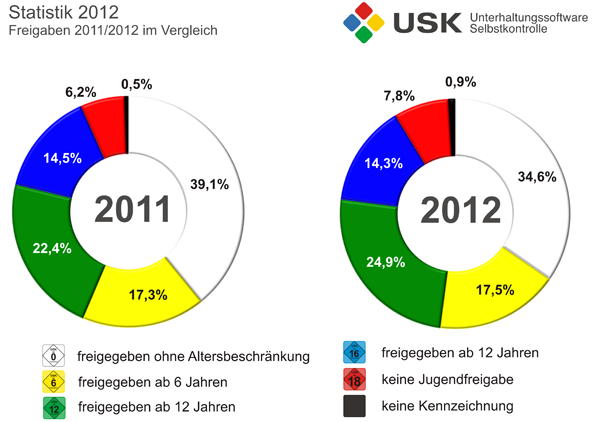
\includegraphics[width=0.8\textwidth]{images/uskfreigaben2012}
\caption[http://www.usk.de/pruefverfahren/statistik/]{Statistik der USK}
\label{uskfreigaben2012}
\end{figure}

Die Statistik der USK zeigt, dass heute ebenfalls viele Spiele f�r Jugendliche ungeeignete Darstellungen von
Gewalt enthalten. 2012 erhielten 8,7 Prozent der gepr�ften Spiele keine Freigabe f�r Jugendliche.


\subsection{Altersfreigaben}
Spiele, die Gewalt (meist in Form von Kampfhandlungen) enthalten, gibt es gleicherma�en in den USK-Alterseinteilungen
"ab 12", "ab 16", "keine Jugendfreigabe" sowie bei Spielen, f�r die die USK die Kennzeichnung verweigerte (Siegel "keine
Kennzeichnung"). Den Unterschied zwischen den ersten drei Stufen macht vor allem der Realit�tsgrad, die
�bertragbarkeitauf die Realit�t und den Alltag, sowie der auf den Spieler ausge�bte Druck, gewaltt�tige Handlungen zu
vollziehen, aus. Das Siegel "Keine Kennzeichnung", das fast immer eine Indizierung durch die BPjM nach sich zieht,
bedeutet dagegen,

\begin{itemize} 
  \item dass Spielinhalte Gewalttaten in der Alltagswirklichkeit legitimieren und Parallelen zur Realit�t nahelegen;
  \item dass das Spiel nur erfolgreich beendet werden kann, wenn Spielfiguren eliminiert werden, die nicht als Gegner auftreten;
  \item dass drastisch inszenierte und grafisch detailliert aufbereitete Gewalttaten gegen menschlich oder menschen�hnlich gestaltete Spielfiguren die Spielhandlung pr�gen;
  \item dass Kriegsbegeisterung vermittelt und Gewaltfolgen explizit bagatellisiert werden.\cite{uskalterskennzeichen}
\end{itemize} 

Das bedeutet, dass Gewalt in Spielen, zumindest laut der Einsch�tzung der Bundespr�fstelle f�r jugendgef�hrdende Medien
(BPjM), nicht zwingend jugendgef�hrdend sein muss, dies aber je nach Darstellung und Rahmenbedingungen sein kann.

\subsection{Gr�nde}
Man k�nnte annehmen, das h�ufige Auftreten von Gewaltdarstellungen in Spielen w�re historisch bedingt. Forschungen im
Bereich der Computertechnik wurden von Beginn an vom Milit�r forciert und finanziert. Das legt nahe, dass milit�rische
Simulationen die Inspiration zu den ersten Computerspielen waren, woraufhin sich der Bezug zur Gewalt einfach bis heute
erhalten haben k�nnte. Die Geschichte spricht jedoch dagegen, wie weiter oben bereits dargestellt. Der erste Shooter der
Welt war gewaltfrei und entwickelt von einem Studenten. Die andauernde Pr�senz von Gewalt in Computerspielen muss als
einen anderen Grund haben.\\

Kunczik und Zipfel haben die verschiedenen Erkl�rungsans�tze dazu gesammelt. Eine dieser Theorien sieht den Reiz von
virtuellen Gewaltszenen in ihrer �sthetischen Wirkung durch Ger�usche, Bewegungen und Farben.\cite{kunczik}

\subsection{Wirkung}
�ber die Wirkung von Gewaltdarstellungen in Computerspielen bzw. in Medien allgemein gehen die Meinungen stark auseinander.
